%% LyX 2.1.3 created this file.  For more info, see http://www.lyx.org/.
%% Do not edit unless you really know what you are doing.
\documentclass[10pt]{beamer}\usepackage[]{graphicx}\usepackage[]{color}
%% maxwidth is the original width if it is less than linewidth
%% otherwise use linewidth (to make sure the graphics do not exceed the margin)
\makeatletter
\def\maxwidth{ %
  \ifdim\Gin@nat@width>\linewidth
    \linewidth
  \else
    \Gin@nat@width
  \fi
}
\makeatother

\definecolor{fgcolor}{rgb}{0.345, 0.345, 0.345}
\newcommand{\hlnum}[1]{\textcolor[rgb]{0.686,0.059,0.569}{#1}}%
\newcommand{\hlstr}[1]{\textcolor[rgb]{0.192,0.494,0.8}{#1}}%
\newcommand{\hlcom}[1]{\textcolor[rgb]{0.678,0.584,0.686}{\textit{#1}}}%
\newcommand{\hlopt}[1]{\textcolor[rgb]{0,0,0}{#1}}%
\newcommand{\hlstd}[1]{\textcolor[rgb]{0.345,0.345,0.345}{#1}}%
\newcommand{\hlkwa}[1]{\textcolor[rgb]{0.161,0.373,0.58}{\textbf{#1}}}%
\newcommand{\hlkwb}[1]{\textcolor[rgb]{0.69,0.353,0.396}{#1}}%
\newcommand{\hlkwc}[1]{\textcolor[rgb]{0.333,0.667,0.333}{#1}}%
\newcommand{\hlkwd}[1]{\textcolor[rgb]{0.737,0.353,0.396}{\textbf{#1}}}%

\usepackage{framed}
\makeatletter
\newenvironment{kframe}{%
 \def\at@end@of@kframe{}%
 \ifinner\ifhmode%
  \def\at@end@of@kframe{\end{minipage}}%
  \begin{minipage}{\columnwidth}%
 \fi\fi%
 \def\FrameCommand##1{\hskip\@totalleftmargin \hskip-\fboxsep
 \colorbox{shadecolor}{##1}\hskip-\fboxsep
     % There is no \\@totalrightmargin, so:
     \hskip-\linewidth \hskip-\@totalleftmargin \hskip\columnwidth}%
 \MakeFramed {\advance\hsize-\width
   \@totalleftmargin\z@ \linewidth\hsize
   \@setminipage}}%
 {\par\unskip\endMakeFramed%
 \at@end@of@kframe}
\makeatother

\definecolor{shadecolor}{rgb}{.97, .97, .97}
\definecolor{messagecolor}{rgb}{0, 0, 0}
\definecolor{warningcolor}{rgb}{1, 0, 1}
\definecolor{errorcolor}{rgb}{1, 0, 0}
\newenvironment{knitrout}{}{} % an empty environment to be redefined in TeX

\usepackage{alltt}
\usepackage{etex}

\usepackage[T1]{fontenc}
\usepackage{textpos} 
\usepackage{hyperref}
\usepackage{amsmath,amsthm,amsfonts,nicefrac,mathabx,amssymb}
\usepackage[subnum]{cases}
\usepackage{calligra, mathrsfs}
%\usepackage{natbib}
\usepackage{booktabs}
%\bibpunct{(}{)}{;}{a}{,}{,}
\usepackage[english]{babel}
\usepackage[latin1]{inputenc}
\usepackage{helvet}
\usepackage{graphicx}
\usepackage{color}
\usepackage{multirow,dcolumn}
\usepackage{ragged2e}
\usepackage{xcolor}
\usepackage{colortbl}
\usepackage{booktabs}
\usepackage{url}
\usepackage{bibentry}
\usepackage{chngcntr}

\ifx\hypersetup\undefined
  \AtBeginDocument{%
    \hypersetup{unicode=true,pdfusetitle,
 bookmarks=true,bookmarksnumbered=false,bookmarksopen=false,
 breaklinks=false,pdfborder={0 0 0},backref=false,colorlinks=false}
  }
\else
  \hypersetup{unicode=true,pdfusetitle,
 bookmarks=true,bookmarksnumbered=false,bookmarksopen=false,
 breaklinks=false,pdfborder={0 0 0},backref=false,colorlinks=false}
\fi

\colorlet{tablesubheadcolor}{gray!25}
\colorlet{tableheadcolor}{gray!40}
\colorlet{tablerowcolor}{gray!15.0}
\usetheme{Gesis}
%\setbeamertemplate{navigation symbols}{}
\setbeamertemplate{footline}[frame number]%{\hspace*{.2cm}\insertframenumber}
\setbeamerfont{caption}{size=\footnotesize}
\usefonttheme[onlylarge]{structuresmallcapsserif} % alte Schrift


\definecolor{hellgrau}{rgb}   {0.109375,  0.40625,   0.51953125}
\definecolor{dunkelgrau}{rgb} {0.009375,  0.30625,   0.41953125}
\definecolor{dunkelgrau2}{rgb}{0.009375,  0.20625,   0.31953125}
\definecolor{hellbraun}{rgb}  {0.9140625, 0.8984375, 0.8046875}
\definecolor{hellbraun2}{rgb} {.95,       0.9,       0.8}
\definecolor{alertred}{rgb}   {0.8515625, 0.3828125, 0.08984375}
\definecolor{orange}{rgb}{1,0.5,0}


\setbeamercolor{firstsecslide}{fg=white,bg=dunkelgrau}
\setbeamertemplate{blocks}[rounded][shadow=true]


\newcommand{\emphred}[1]{\textcolor{alertred}{#1}}
\newcommand{\emphcol}[1]{\textcolor{dunkelgrau}{\slshape #1}}

\newcommand{\eqname}[1]{\tag*{#1}} %equation title

\newenvironment{frcseries}{\fontfamily{frc}\selectfont}{}
\newcommand{\textfrc}[1]{{\frcseries#1}}
\newcommand{\mathfrc}[1]{\text{\textfrc{#1}}}


\setcounter{tocdepth}{1}
\setbeamercolor*{section in toc}{fg=hellgrau}
\setbeamertemplate{bibliography item}[default]


\setcounter{secnumdepth}{3}
\setcounter{tocdepth}{3}


\newcommand{\E}[1]{\text{E}\left(#1\right)}
\newcommand{\V}[1]{\text{V}\left(#1\right)}
\newcommand{\Vest}[1]{\widehat{\text{V}}\left(#1\right)}
\newcommand{\MSE}[1]{\text{MSE}\left(#1\right)}
\newcommand{\COV}[2]{\text{COV}\left(#1,\,#2\right)}

\makeatletter

%%%%%%%%%%%%%%%%%%%%%%%%%%%%%% LyX specific LaTeX commands.
\providecommand{\LyX}{\texorpdfstring%
  {L\kern-.1667em\lower.25em\hbox{Y}\kern-.125emX\@}
  {LyX}}

%%%%%%%%%%%%%%%%%%%%%%%%%%%%% Textclass specific LaTeX commands.
% this default might be overridden by plain title style
 \newcommand\makebeamertitle{\frame{\maketitle}}%
 % (ERT) argument for the TOC
 \AtBeginDocument{%
   \let\origtableofcontents=\tableofcontents
   \def\tableofcontents{\@ifnextchar[{\origtableofcontents}{\gobbletableofcontents}}
   \def\gobbletableofcontents#1{\origtableofcontents}
 }

%%%%%%%%%%%%%%%%%%%%%%%%%%%%%% User specified LaTeX commands.
%\usetheme{Montpellier}%\usetheme{PaloAlto}

\makeatother

\addtobeamertemplate{frametitle}{}{%
\begin{textblock*}{100mm}(.91\textwidth,-1cm)

\includegraphics[height=1cm,width=2cm]{graphs/logos/GESIS_Logo_kompakt_en.jpg}
\end{textblock*}}
\IfFileExists{upquote.sty}{\usepackage{upquote}}{}
\begin{document}




\title[Sampling Designs]{Sampling and Estimation}   
\subtitle{Day 1: Sampling Designs}

\author{Stefan Zins\thanks{\href{mailto:Stefan.Zins@gesis.org}{Stefan.Zins@gesis.org}} and Matthias Sand\thanks{\href{mailto:Matthias.Sand@gesis.org}{Matthias.Sand@gesis.org}}}
\date{\today} 

\makebeamertitle

\section{Welcome and Introduction}

\begin{frame}{Objectives  of the Course}
\Large
  \begin{itemize}
  \item<1-|alert@1> Understanding the basic principles  of design-based inference, \vspace{1cm}
  \item<2-|alert@2> apply them to estimated form complex survey samples  (or the planning of surveys), and \vspace{1cm}
  \item<3-|alert@3> learn how to do this with R!
  \end{itemize}
\end{frame}

\begin{frame}{Motivation}

  \begin{itemize}
    \item<1-2,3-> \only<1,3,4>{What do you want to do?} 
    \only<2>{\begin{center} 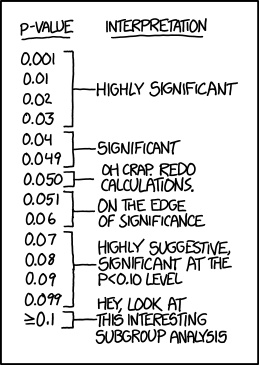
\includegraphics[width=5cm]{graphs/p_values.png} \\{ \footnotesize Source:  \href{http://xkcd.com/1478/}{http://xkcd.com/1478/} }  \end{center}}     \vspace{1cm}
    \item<3-> How do you plan on doing it?  \vspace{1cm}
    \item<4>  What problems do you foresee?
  \end{itemize}
\end{frame}


\begin{frame}{Finite population, Sample, and Sampling Design}

 \begin{itemize}
 \item[] 
 \begin{align}
 \mathcal{Y} = & \{ y_1{,}y_2{,}\,\ldots{,}\,y_k{,}\,\ldots{,}\,y_N \} \eqname{finite population of size $N$} \\
 \mathcal{U} = &\, \{ 1{,}2{,}\,\ldots{,}\,k{,}\,\ldots{,}\,N \} \eqname{sampling frame} \\
 \mathfrc{s} \subset &\, \mathcal{U} \eqname{sample of size $n$} \\
 \mathcal{P}(\mathcal{U}) & \eqname{all possible subsets of $\mathcal{U}$}
 \end{align}
 \item[]
\item[]
The discrete probability distribution $p(.)$ over $\mathcal{P}(\mathcal{U})$ is called
a \emph{sampling design} and  $\mathcal{G}=\{ \mathfrc{s} | \mathfrc{s} \in
\mathcal{P}(\mathcal{U}),\, p(\mathfrc{s}) > 0 \}$ is called the support of $p(.)$ with
$$
\sum_{\mathfrc{s} \in \mathcal{G}} p(\mathfrc{s}) = 1
$$
Hence, $p: \; \mathcal{G} \mapsto (0, 1]$.
 \end{itemize}
\end{frame}


\begin{frame}{Estimation}
\begin{align}
 \theta       & = f(\mathcal{Y})  \eqname{statistic of interest} \\
 \hat{\theta} & = f(\mathcal{Y}, \mathfrc{s} )  \eqname{estimator for $\theta$} \\
 \E{\hat{\theta}} & = \sum_{\mathfrc{s} \in \mathcal{G}} p(\mathfrc{s}) f(\mathcal{Y}, \mathfrc{s} )   \eqname{expected value of $\hat{\theta}$} \\
 \V{\hat{\theta}}   & =  \E{\hat{\theta}^2} -  {\E{\hat{\theta}}}^2 \eqname{variance of  $\hat{\theta}$} \\
 \MSE{\hat{\theta}} & = \E{(\hat{\theta} - \theta)^2} \nonumber \\
                    & = \left(\E{\hat{\theta}} - \theta\right)^2 + \V{\hat{\theta}} \eqname{mean square error of $\hat{\theta}$}
\end{align}
 $\E{.}$, $\V{.}$, and $\MSE{.}$ are always with respect to the sampling design $p()$ and
 an estimator is said to be unbiased if
 $$ \E{\hat{\theta}} = \theta\;. $$
\end{frame}


\begin{frame}{Representative Sample}
\onslide*<1-2>{What is a representative sample? \newline}
\onslide*<2>{The popular concept of a representative sample it that the sample is a \emph{miniature} of the population.}

\onslide<3-4>{However, what do we really want?}
\onslide<4>{\newline We want to estimate a statistic of interest with a certain level of precision 
 and if the level of precision is high enough we say our estimation \emph{strategy} is representative.}

\end{frame}

\begin{frame}{Strategy}
A \emph{strategy} is the combination of a sampling design and an estimator.
For the statistic of interest the aim is to find the best possible strategy, that is, one that estimates the statistic as accurately as possible.

A measure of accuracy can be the mean square error.

\end{frame}

\begin{frame}{Expectation and Variance \\ of a Random Sample}
\begin{align}
 S_k   &    \eqname{number of times element $k$ is selected} \\
 I_k   &=   \begin{cases}   1  & \text{if}\; k \in \mathfrc{s} \\
                            0  & \text{else}  
          \end{cases}   \eqname{sampling indicator element $k$} \\
\E{S_k}     &  =  \nu_k    \eqname{expected selection frequency of element $k$} \\
\E{S_k S_l} &  =  \nu_{kl} \eqname{joint expectation  of $S_k$ and $S_l$} \\
\E{I_k}     &  =   \pi_k    \eqname{inclusion probability of element $k$ } \\
\E{I_k I_l} &  =   \pi_{kl}  \eqname{joint expectation of $I_k$ and $I_l$} 
\end{align}
\begin{equation}
\sum_{k \in \mathcal{U}}\nu_k = \E{n} \eqname{expected sample size}
\end{equation}
\end{frame}



\begin{frame}{Simple Random Sampling}{Without Replacement}
Simple random sampling without replacement (SRS):
Drawing $n$ elements out of a urn without putting them back (i.e. $S_k=I_k$) and without remembering the order of the selected element.
\begin{align}
  \mathcal{G}    =&  \binom{N}{n}         \\
  p(\mathfrc{s}) =& {\binom{N}{n}}^{-1} \\
  \pi_k =\nu_k  =&  \dfrac{n}{N} \\
  \pi_{kl} =\nu_{kl}  =&  \dfrac{n(n-1)}{N(N-1)}\; \text{for}\; k \neq l
\end{align}
\end{frame}

\begin{frame}{Sample Mean with SRS}
  ~\\[-1cm]
  \begin{align*} 
  \theta  =\mu = \dfrac{1}{N} \sum_{k \in \mathcal{U}}  y_k{,}  && \hat{\theta} = \overline{y} = \sum_{k \in \mathfrc{s}}  \dfrac{y_k}{n}{,} && \sigma^2 = \dfrac{1}{N}\sum_{k \in \mathcal{U}} (y_k - \mu )^2{,}
  && V^2 = \sigma^2 \dfrac{N}{N-1}
  \end{align*}
  \begin{columns}[t]
   \onslide<2->{
    \begin{column}{.5\textwidth}
    Expected value
      \begin{align*} 
        \E{\overline{y}} & = \E{\sum_{k \in \mathcal{U}} S_k \dfrac{y_k}{n} } \\
        & = \dfrac{1}{n} \sum_{k \in \mathcal{U}} \E{S_k} y_k  \\
        & = \dfrac{1}{n} \sum_{k \in \mathcal{U}} \pi_k y_k  \\
        & = \dfrac{1}{N} \sum_{k \in \mathcal{U}}  y_k  
       \end{align*}
      \end{column}
    \begin{column}{.5\textwidth}
   }
   \onslide<3>{
    Variance
      \begin{align*} 
        \V{\overline{y}} & = \V{\sum_{k \in \mathcal{U}} S_k \dfrac{y_k}{n}} \\
        & = \dfrac{1}{n^2} \sum_{k \in \mathcal{U}} \sum_{l \in \mathcal{U}} \COV{S_k}{S_l} y_k y_l  \\
        & = -\dfrac{1}{2} \dfrac{1}{n^2} \sum_{k \in \mathcal{U}} \sum_{l \in \mathcal{U}} (\pi_{kl}-\pi_k\pi_l)  \left(y_k - y_l \right)^2  \\
        & = \dfrac{N-n}{N-1} \dfrac{\sigma^2}{n}  =   \left( 1 -  \dfrac{n}{N} \right) \dfrac{V^2}{n}
      \end{align*}
    \end{column}
   }
    \end{columns}
 \end{frame}


\begin{frame}{Simple Random Sampling}{With Replacement}
Simple random sampling with replacement (SRSWR):
Drawing $n$ elements out of a urn by making $n$ successive draws and putting after each draw the element back (i.e. $S_k \neq I_k$). The order of the selected elements is also not remembered.
\begin{align*}
  \mathcal{G}= & \binom{N+n-1}{n}     &  p(\mathfrc{s}) = & {\binom{N+n-1}{n}}^{-1}   \\
 \nu_k      = & \dfrac{n}{N}         &  \pi_k          = &  1-\left( \dfrac{N-1}{N} \right)^n \\
 \nu_{kl}   = & \dfrac{n(n-1)}{N^2}  &  \pi_{kl}       = &  1- 2\left( \dfrac{N-1}{N}  \right)^n + \left( \dfrac{N-2}{N}  \right)^n \qquad \text{for}\; k \neq l
\end{align*}
\end{frame}


\begin{frame}{Sample Mean with SRSWR}
  \begin{columns}[t]
   \onslide<1->{
    \begin{column}{.5\textwidth}
    Expected value
      \begin{align*} 
        \E{\overline{y}} & = \E{\sum_{k \in \mathcal{U}} S_k \dfrac{y_k}{n} } \\
        & = \dfrac{1}{n} \sum_{k \in \mathcal{U}} \E{S_k} y_k  \\
        & = \dfrac{1}{n} \sum_{k \in \mathcal{U}}\nu_k y_k  \\
        & = \dfrac{1}{N} \sum_{k \in \mathcal{U}}  y_k  
       \end{align*}
      \end{column}
    \begin{column}{.5\textwidth}
   }
   \onslide<2->{
    Variance
      \begin{align*} 
        \V{\overline{y}} & = \V{\sum_{k \in \mathcal{U}} S_k \dfrac{y_k}{n}} \\
        & = \dfrac{1}{n^2} \sum_{k \in \mathcal{U}} \sum_{l \in \mathcal{U}} \COV{S_k}{S_l} y_k y_l  \\
        & = -\dfrac{1}{2} \dfrac{1}{n^2} \sum_{k \in \mathcal{U}} \sum_{l \in \mathcal{U}} (\nu_{kl}-\nu_k\nu_l)  \left(y_k - y_l \right)^2  \\
        & = \dfrac{\sigma^2}{n}    
      \end{align*}
    \end{column}
   }
    \end{columns}
    \onslide<3>{\begin{center} 
     Note: $\dfrac{\sigma^2}{n} >   \left( 1 -  \dfrac{n}{N} \right) \dfrac{V^2}{n}$, if $n > 1$.
     \end{center}}
 \end{frame}

\begin{frame}{Variance Estimation SRS/WR}
\begin{align*}
\Vest{\overline{y}}_{\text{SRS}}   =   \dfrac{N-n}{N} \dfrac{s^2}{n} \\
\Vest{\overline{y}}_{\text{SRSWR}} =  \dfrac{s^2}{n} 
\end{align*}
Sample variance
\begin{equation*}
s^2 = \dfrac{1}{n-1} \sum_{k \in \mathfrc{s}} (y_k - \overline{y})^2 = \dfrac{1}{n(n-1)} \sum_{k \in \mathcal{U}} \sum_{l \in \mathcal{U}} (y_k - y_l)^2 S_k S_l
\end{equation*}
\begin{align*}
\E{s^2}_{\text{SRS}}    &=   \dfrac{N}{N-1} \sigma^2 = V^2 \\
\E{s^2}_{\text{SRSWR}}  &=   \sigma^2
\end{align*}

\end{frame}

\begin{frame}{Model-based Approach}
The sample data: $\mathfrc{y}=\{y_1{,}\,\ldots{,}\,y_k{,}\,\ldots{,}\,y_n\}$.
All $y_k \in \mathfrc{y}$ are independent identical distributed (iid) random variables, with
\begin{equation*}
  y_k \sim NV(\mu, \sigma)\;{.}
\end{equation*}
\begin{columns}[t]
   \onslide<2->{
    \begin{column}{.5\textwidth}
    Expected value
      \begin{align*} 
        \E{\overline{y}}_{M} & = \E{\sum_{k \in \mathfrc{s}} \dfrac{y_k}{n} } \\
        & = \dfrac{1}{n} \sum_{k \in \mathfrc{s}} \mu  \\
        & = \mu
       \end{align*}
      \end{column}
    \begin{column}{.5\textwidth}
   }
   \onslide<3->{
    Variance
      \begin{align*} 
        \V{\overline{y}}_{M} & = \V{\sum_{k \in \mathfrc{s}} \dfrac{y_k}{n}}_{M} \\
        & = \dfrac{1}{n^2} \sum_{k \in \mathfrc{s}} \sigma^2 \\
        & = \dfrac{\sigma^2}{n}    
      \end{align*}
    \end{column}
   }
    \end{columns}
     \onslide<4>{Note that the variance of $\overline{y}$ is the same under the model based approach and SRSWR, i.e. there is no finite population correction.}
\end{frame}


\begin{frame}{Features of Sampling Designs}
\begin{itemize}
\item Stratification
\item Cluster Sampling: Not elementary units are selected but \emph{clusters} containing multiple elements. 
\item Multistage Sampling: The population is structured by hierarchically ordered clusters that are nested within each other. The sampling procedure has multiple selecting stages. 
\end{itemize}
\end{frame}


\begin{frame}{StrRS Notation I}
  The universe $\mathcal{U}$ is decomposed into $H$ non-overlapping groups,
  $\mathcal{U}_1,\dots,\mathcal{U}_H$ ,called strata.
  \begin{itemize}
  	\item $\mathcal{U} = \bigcup\limits_{h=1}^H \mathcal{U}_h$, where set $\mathcal{U}_h$ is
  the $h$-th
  strata. 
  	\item A sample $\mathfrc{s}_{h}$ is selected from $\mathcal{U}_h$ according to a design
  $p_h(\ldotp)$, for all $h=1,\,\ldots,\,H$. 
  	\item The number of elements in $\mathcal{U}_h$ is called stratum size and denote
  with $N_h$
  	\item The number of elements in $\mathfrc{s}_{h}$ is denoted with $n_h$.
  \end{itemize}
\end{frame}

\begin{frame}{Stratified Random Sampling Notation II}
  In stratified random sampling the sub-populations are called strata. For the  $h$-ht stratum
  we get:
  
  \begin{align}
  \mu_{h}      &= \frac{1}{N_h} \sum^{N_h}_{k=1} y_{kh} \eqname{mean of stratum h} \\
  \sigma^2_{h} &= \frac{1}{N_h}\sum^{N_h}_{k=1} (y_{kh}-\mu_{h})^2  \eqname{variance of stratum $h$} \\
  V^2_{h} & = \sigma^2_{h} \dfrac{N_h}{N_h-1} \nonumber
  \end{align}
  
  Where  $y_{kh}$ as the $k$-th element in the $h$-th stratum.
  Sampling from stratified populations is called stratified random sampling (StrRS).
  
\end{frame}


\begin{frame}{Stratification}
A Population of 100 elements is stratified into $H=6$ strata.

%fig.keep='all',fig.show='asis'
\onslide*<1>{
\begin{knitrout}\footnotesize
\definecolor{shadecolor}{rgb}{0.969, 0.969, 0.969}\color{fgcolor}

{\centering 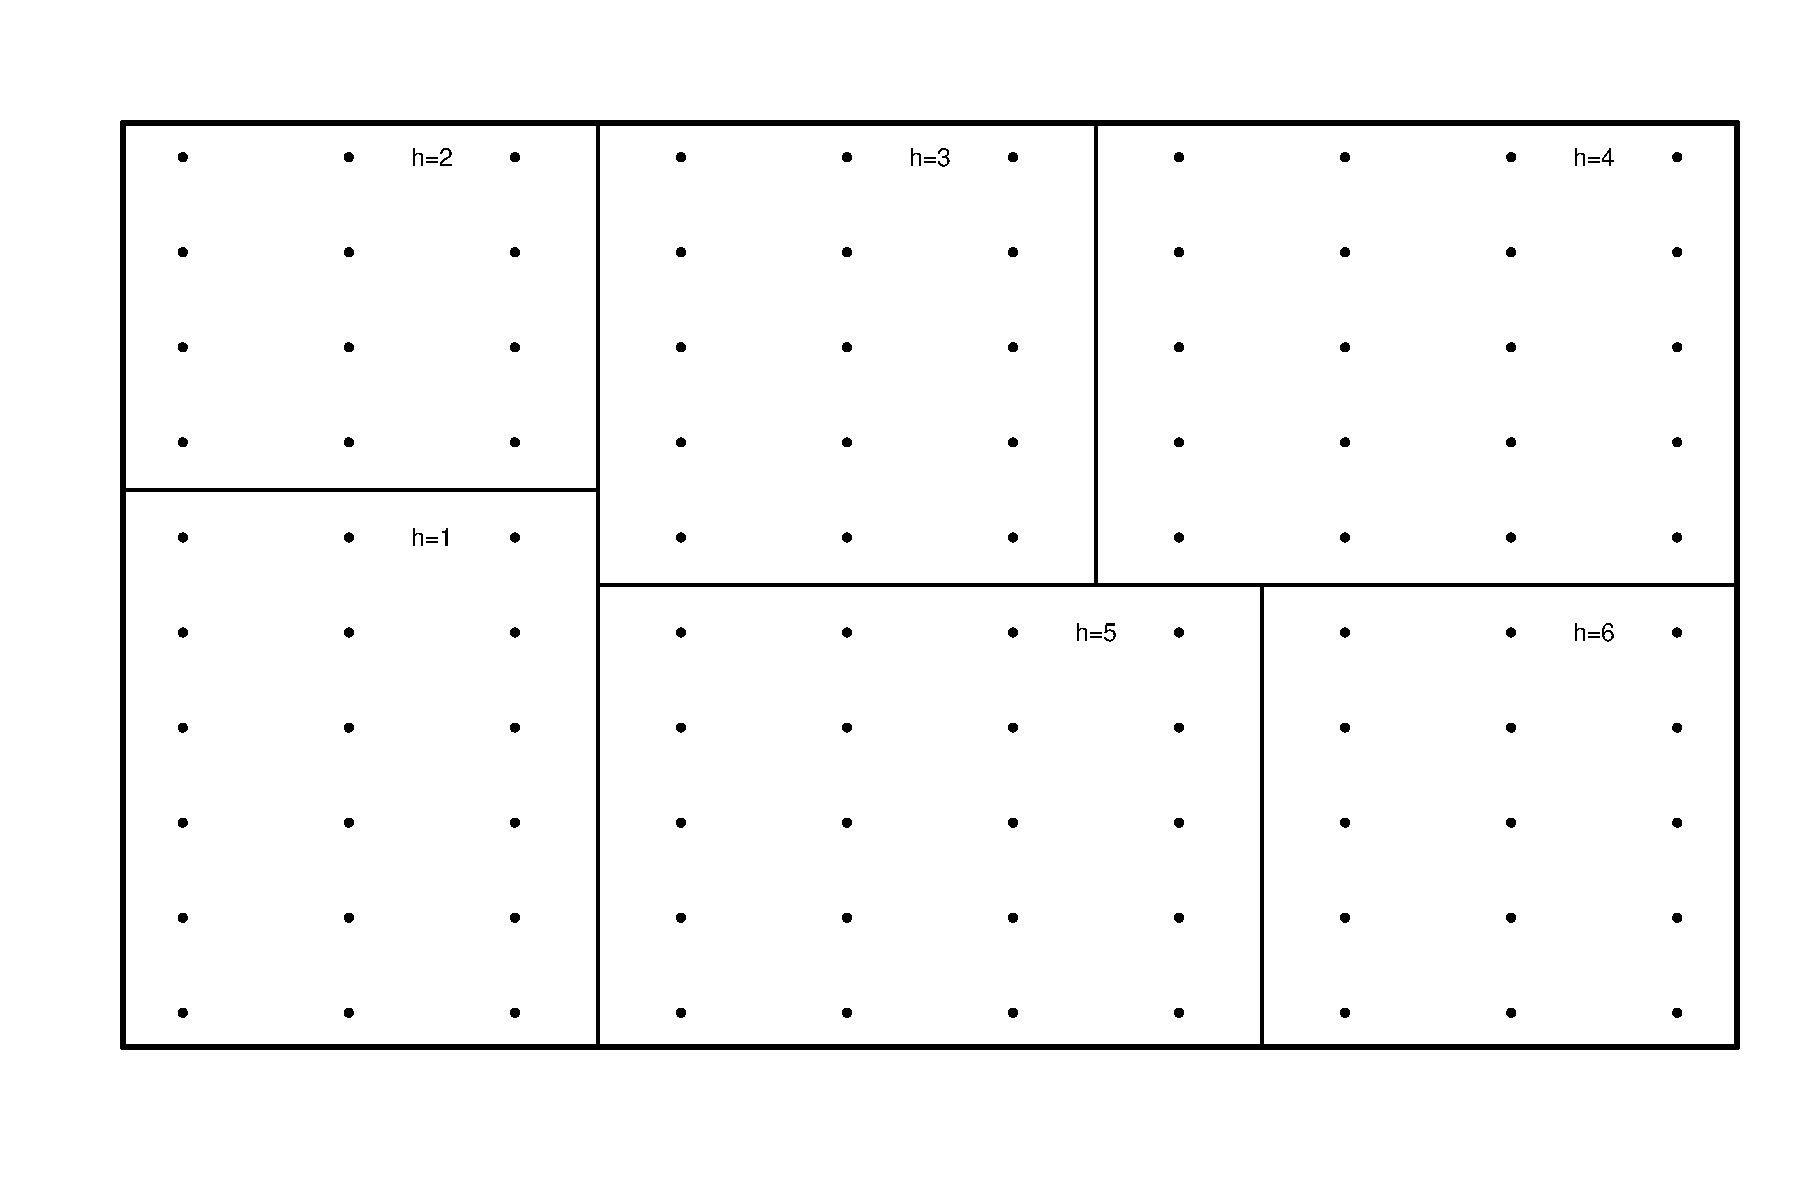
\includegraphics[width=.85\linewidth]{graphs/beamer-StratPlot1-1} 

}



\end{knitrout}
}
\onslide<2>{
14 elements are selected population and their allocation is given by
\begin{tabular}{cccccc}
$n_1$ = 2  & $n_2$ = 3  & $n_3$ = 2  & $n_4$ = 3 & 
 $n_5$ = 3&  $n_6$ = 2\\
\end{tabular}

\begin{knitrout}\footnotesize
\definecolor{shadecolor}{rgb}{0.969, 0.969, 0.969}\color{fgcolor}

{\centering 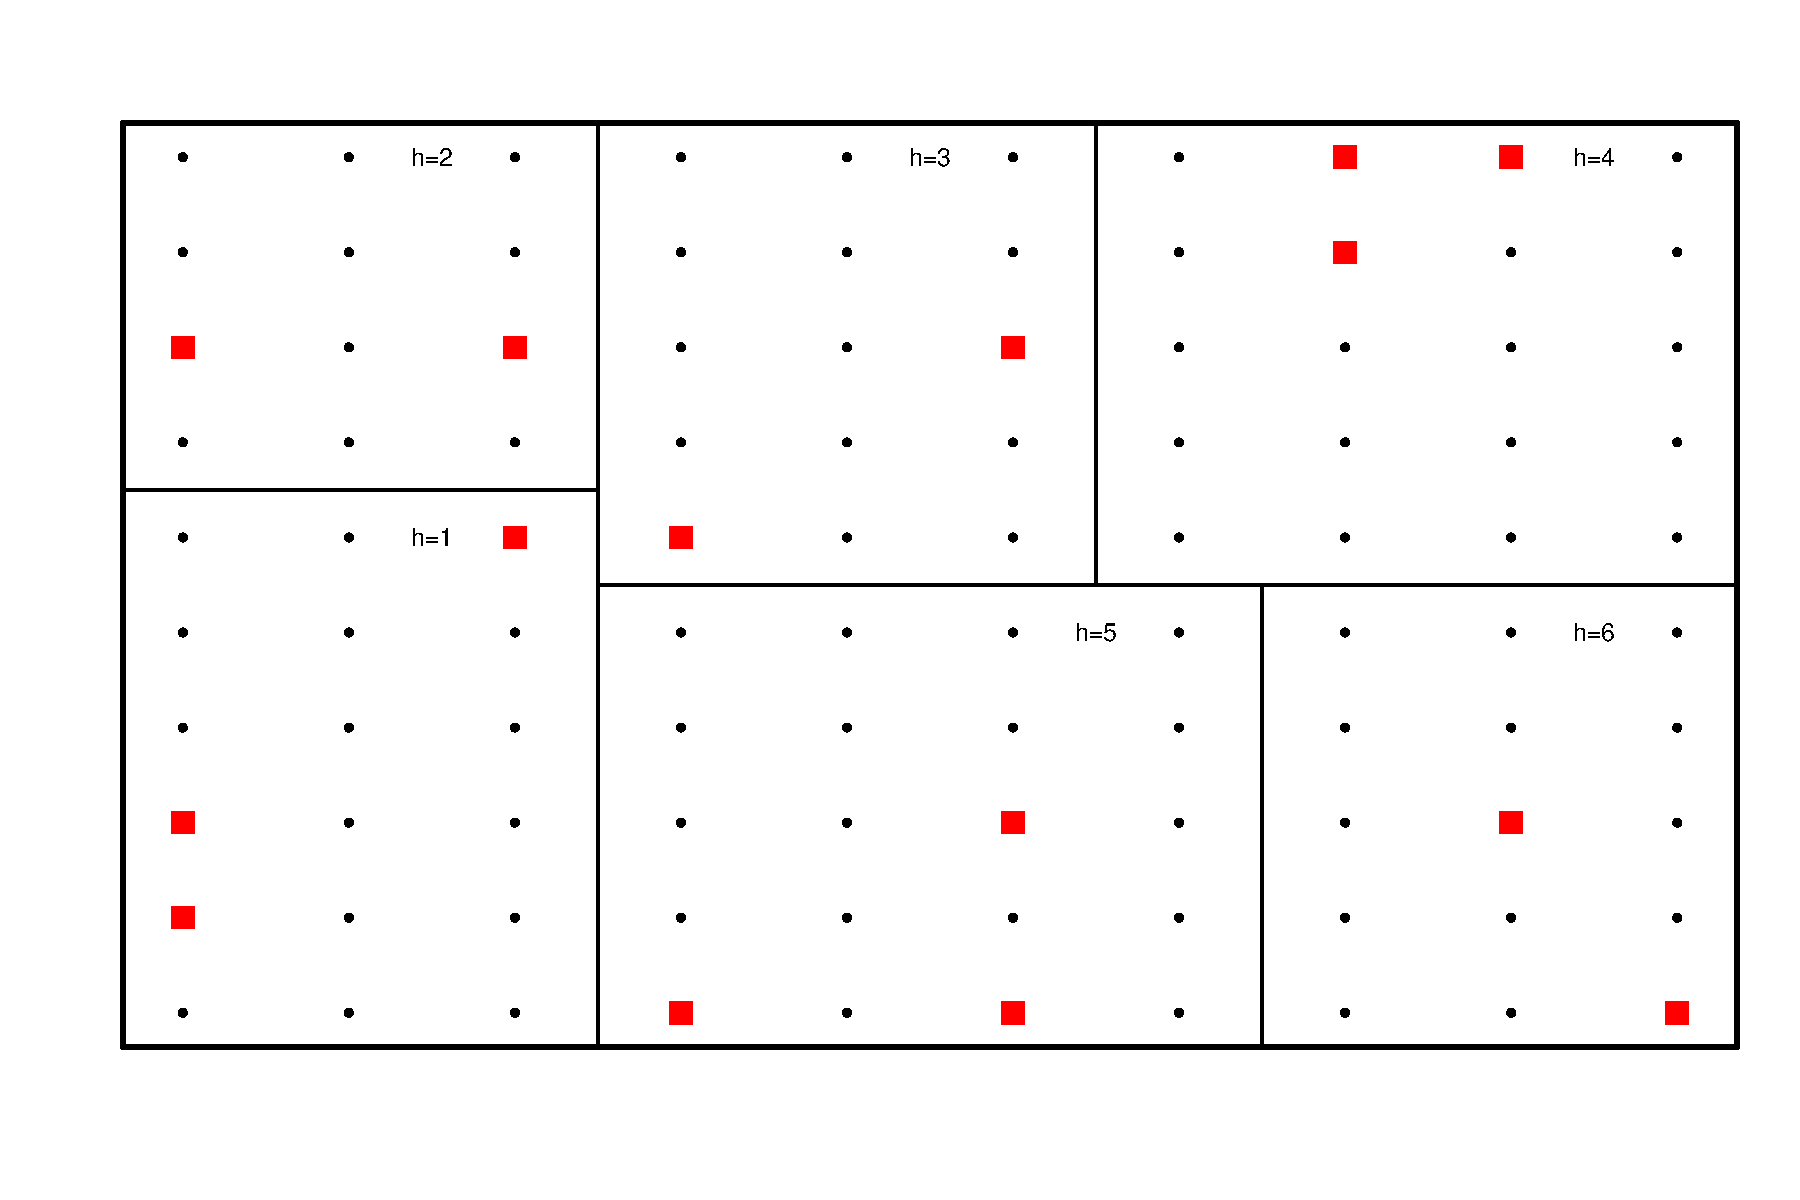
\includegraphics[width=.85\linewidth]{graphs/beamer-StratPlot2-1} 

}



\end{knitrout}
}
\end{frame}

\begin{frame}{Estimation}
  Estimator for the mean:
  \begin{equation*}
  \overline{y}_{\text{str}} = \sum_{h=1}^H \gamma_h \overline{y}_h
  \end{equation*}
  where $\gamma_h = \dfrac{N_h}{N}$ and $\E{\overline{y}_{\text{str}}} = \mu$ for SRS and SRSWR within each stratum.
  \newline
  Variance and variance estimator:
  \begin{align*}
  \V{\overline{y}_{\text{str}}}_{\text{SRS}} & = \sum_{h=1}^H \dfrac{N_h-n_h}{N_h} \gamma_h^2 \dfrac{V_{h}^2}{n_h} \\
  \Vest{\overline{y}_{\text{str}}}_{\text{SRS}} & = \sum_{h=1}^H \dfrac{N_h-n_h}{N_h} \gamma_h^2 \dfrac{s_{h}^2}{n_h} 
  \end{align*}
  \begin{equation*}
  s^2_{h} = \dfrac{1}{n_h-1} \sum_{k \in \mathfrc{s}_h} (y_k - \overline{y}_h)^2
  \end{equation*}

\end{frame}


\begin{frame}{Issues with Stratification}
\begin{itemize}
\item<1-> Why should stratification be used?
\begin{itemize}
\item<2-> To reduce the sampling variance of estimators.
\item<2-> Sometimes it is necessary because of organizational reasons, (e.g. no joint sampling frame).
\end{itemize}
\item<3-> How should the population be stratified?
\begin{itemize}
\item<4-> A \emph{good} set of variables needs to be found for stratification.
\item<4-> The number of strata has to be decided.
\item<5-> (You might check out the \texttt{SamplingStrata} package, it 
implements a method to determine of the best stratification of a sampling frame,
of minimal cost under the condition to satisfy precision constraints in a multivariate and multi-domain case.)
\end{itemize}
\item<6-> How should the overall sample size be allocated to the strata?
\begin{itemize}
\item<7-> Achieve proportionality between sample and population (i.e. the frame)
\item<7-> Fulfill precision constraints for certain estimation domains
\end{itemize}
\end{itemize}

\end{frame}

\begin{frame}{Defining the Strata}
  \begin{table}\caption{Population ANOVA}
  \begin{tabular}{l | l | l }
  Source & df & Sum of Squares  \\
  \hline 
   Between strata         & $H-1$ & $\text{SSB}  = \sum_{h=1}^H N_h ( \mu_{h} - \mu  )^2$  \\ 
   Within  strata         & $N-H$ & $\text{SSW}  = \sum_{h=1}^H (N_h-1) V_{h}^2$  \\
   Total,  about  $\mu_y$ & $N-1$ & $\text{SSTO} = (N-1) V^2$ \\
  \end{tabular}
  \end{table}

The more homogeneous the strata are the higher is the gain in efficiency from using stratified simple random sample sampling (StrSRS) instead of SRS. Because then SSW (variance within) is
considerably small in contrast to SSB (variance between). This is called
the  effect of stratification. 

\end{frame}
% %survey imperfections 
%$N_h > 2$ variance estimation is difficult 
% $\V{\hat{\theta}}$

\section{Allocation Methods}

\begin{frame}{Allocation Methods}
For all $h = 1{,}\,\ldots{,}\,H$
 \begin{equation*} \arraycolsep=1.4pt\def\arraystretch{2.2}
  n_h = \left\{ \begin{array}{l r}
        \dfrac{n}{H}  &\; \text{equal allocation} \\
        \dfrac{N_h}{N}  n    &\; \text{proportional allocation} \\
        \dfrac{N_h V_{h}}{\sum_{h=1}^H N_h V_{h} }  n  &\; \text{optimal allocation} \\
        \dfrac{c}{\overline{c}_h} \dfrac{N_h V_{h} \sqrt{\overline{c}_h} }{\sum_{h=1}^H N_h V_{h} \sqrt{\overline{c}_h}}    &\;  \text{cost-optimal allocation}
  \end{array}\;\right.{,}
 \end{equation*}
 where $\overline{c}_h$ are average cost of selecting a element from stratum $h$ and $c=\sum_{h=1}^H n_h \overline{c}_h$ are the total costs of the survey. For the cost-optimal allocation $c$ is given, not $n$.
% 
% Variants of proportional allocation to totals
% proportional to y or auxiliar variable
% %the rounding probelem
\end{frame}

\begin{frame}{On Proportional Allocation}
If $n_h =  \dfrac{N_h}{N}  n$  
\begin{align*}
\V{\overline{y}_{\text{str}}}_{\text{StrSRS}} & = \left( \dfrac{N - n}{N} \right) \dfrac{1}{n} \sum_{h=1}^H N_h  V_{h}^2\qquad \text{and }\\
\V{\overline{y}}_{\text{SRS}} & = \left( \dfrac{N - n}{N} \right) \dfrac{1}{n(N-1)} \left( \text{SSW} + \text{SSB} \right) \\
& = \V{\overline{y}_{\text{str}}}_{\text{StrSRS}} + \left(\dfrac{N - n}{N}  \right) \dfrac{1}{n(N-1)}\left[ \text{SSB} - \sum_{h=1}^H \dfrac{N - N_h}{N} V^2_{h}  \right]\;.
\end{align*}
Thus, StrSRS with prop. allocation will always result in an equal or smaller variance than SRS if
$$ SSB > \sum_{h=1}^H \dfrac{N - N_h}{N} V^2_{h} \;.$$
\end{frame}


\begin{frame}{The Rounding Problem}
  \begin{itemize}
  \item It is not assured that $\gamma_h n$ is an integer. If 
$n_h^{\ast}=\left[ n_h \right]$ is used instead, the allocation is no longer
strictly proportional. Furthermore $\sum_{h=1}^H n_h^{\ast}=n$ is also not assured.
  \item However stochastic techniques can be used that ensure that $\E{n_h^{\ast}}=n_h$ and
thus $\E{\sum_{h=1}^H n_h^{\ast}}=n$.
 \end{itemize}
  \begin{gather*}
  n_h^{\ast} = \begin{cases} \lfloor n_h \rfloor & \mbox{with prob. } 1 - (n_h \mod{1}) \\
			    \lceil  n_h \rceil  & \mbox{with prob. } (n_h \mod{1})
                \end{cases} 
 \end{gather*}
There are stochastic rounding procedures that are controlled and unbiased, i.e. $\sum_{h=1}^H n_h =n$ and  $\E{n^{\ast}_h} = \frac{N_h}{N} n$ and $|n^{\ast}_{h} - n_{h}| \leq 1$ [Cox, 1987].
\end{frame}


%Variants of proportional allocation to totals
% The rounding problem:
% For SRS within each stratum and exact proportional allocation $\pi_k = \frac{n}{N}$ for all $k \in \mathcal{U}$.
% Problem: There is no guarantee that $\frac{N_h}{N}n$ is a integer. This rounding problem can be negiliable for large $N_h$
% There a stochastic rounding procedures that are controlled and unbiased, i.e. $\sum_{h=1}^H n_h =n$ and  $\E{n_h} = \frac{N_h}{N} n$. [Cox]



\begin{frame}{Simple Systematic Sampling}
 The elements of a population of size $N=n H$ are ordered in a specific way (every unit having a unique rank).
 Starting form a random number $k$, with $1 \leq k \leq H$ and $ k\in \{ 1{,}2{,}\,\ldots{,}\,H \}$ the sample is defined as the elements with ranks 
 $$k{,}\, k+H{,}\, k+2H{,}\,k+3H{,}\,\ldots{,}\, k+(n-1)H\,{.}$$
 %The design has $H$ possible non-overlapping samples.
 %Picture?
\begin{align*}
\overline{y}_{k} & = \dfrac{1}{n} \sum_{i=0}^{n-1} y_{(k+iH)}   \eqname{sample mean}        \\
 \E{\overline{y}_{k}}_{\text{SyS}} &= \mu  \eqname{expected value of $\overline{y}_{k}$} \\
 \V{\overline{y}_{k}}_{\text{SyS}} &=  \dfrac{1}{H} \sum_{h=1}^H \left( \overline{y}_{k} - \mu  \right)^2  \eqname{variance of $\overline{y}_{k}$}
\end{align*}
%right?
There is no unbiased variance estimator for systematic sampling.
Ordering the population with respect to certain variables has a 
similar effects as stratification by the same variable with proportional allocation.
\end{frame}


%' \begin{frame}{Selecting a Sample Size}
%' The sample size can be set to achieve a desired level of precision in terms of the variance 
%' $\V{\hat{\theta}}$ or the variation coefficient $\text{CV}(\hat{\theta})  = \frac{\sqrt{\text{V}_0(\hat{\theta})}}{\hat{\theta}}$. \newline
%' Set $\text{CV}(\overline{y}) = \text{CV}_0$ as a precision requirement (representative!).
%' \begin{align}
%' n & = \dfrac{ V^2  \mu^{-2}}{\text{CV}_0^2 +  V^2  N^{-1} \mu^{-2}} \eqname{SRS} \\
%' n & = \dfrac{ \sigma^2  \mu^{-2}}{\text{CV}_0^2} \eqname{SRSWR}
%'  \end{align}
%' \end{frame}
%' 
%' \begin{frame}{Sample Size for Proportions}
%' \onslide*<1,3>{If the variable of interest is binary we have $\V{\overline{y}}_{\text{SRS}} = \dfrac{\mu(1-\mu) }{n} \dfrac{N-n}{N-1}$
%' and $\text{CV}^2(\overline{y})_\text{SRS}=\left( \dfrac{1}{n} - \dfrac{1}{N}\right) \dfrac{N}{N-1} \dfrac{(1-\mu)}{\mu}$
%' However
%' $$ \lim_{\mu \to 0} \text{CV}^2(\overline{y})_\text{SRS} = \infty\;, $$
%' thus for rare observation to meet a CV target the sample size can become very large.
%' }
%' \onslide*<2>{
%' <<SamSizeSRSprobs,echo=FALSE,fig.width=12,fig.height=8,out.width='.85\\linewidth',message=FALSE,warning=FALSE,fig.cap="Sample Sizes to Achieve CV's of 0.05 and 0.01 for N=50000">>=
%'  CV_01 <- 0.05
%'  CV_02 <- 0.01
%'  p <- seq(0.001, 0.999, length.out = 100)
%'  N <- 50000
%' 
%'  n_01 <- nProp(CV0 = CV_01,pU = p,N = N)
%'  n_02 <- nProp(CV0 = CV_02,pU = p,N = N)
%'  
%'  plot(x=p ,y=n_01,type="l",lwd=3,ylab="n",panel.first = grid(lwd=3),cex.lab=2, cex.axis=2,ylim=c(range(n_02)),xlab=expression(mu) )
%'  lines(x=p,y=n_02,lwd=3, type="l", lty=2)
%'  legend(0.7, max(n_02), c("CV=0.05","CV=0.01"), cex=2, lty=1:2,lwd=2)
%' @
%' }
%' \onslide*<3>{Target values for $\V{\overline{y}}_{\text{SRS}}$  can  instead be set to achieve a CI's with a maximal length of $2\epsilon$ and we select the sample size the following way
%' \begin{align*}
%' \epsilon \geq & z_{1-\alpha/2} \sqrt{ \dfrac{\mu(1-\mu) }{n} \dfrac{N-n}{N-1} } \\
%' n \geq & \dfrac{ z_{1-\alpha/2}^2 \frac{N}{N-1} \mu(1-\mu) }{\epsilon^2  + \frac{1}{N}  z_{1-\alpha/2}^2 \frac{N}{N-1} \mu(1-\mu) }
%' \end{align*}
%' }
%' \onslide<4>{
%'  <<SamSizeSRSprobs2,echo=FALSE,fig.width=12,fig.height=8,out.width='.85\\linewidth',message=FALSE,warning=FALSE,fig.cap="Sample Sizes to Achieve Absolute Errors of 0.05 and 0.01 for N=50000">>=
%'  e_01 <- 0.05
%'  e_02 <- 0.01
%'  p <- seq(0.001, 0.999, length.out = 100)
%'  N <- 50000
%'  z <- qnorm(1-0.05/2)
%'  n_01 <- (N/(N-1)*z^2*p*(1-p))/(e_01^2+z^2*p*(1-p)/(N-1))
%'  n_02 <- (N/(N-1)*z^2*p*(1-p))/(e_02^2+z^2*p*(1-p)/(N-1))
%'  
%'  plot(x=p ,y=n_02,type="l",lwd=3,ylab="n",panel.first = grid(lwd=3),cex.lab=2, cex.axis=2,lty=2,xlab=expression(mu) )
%'  lines(x=p,y=n_01,lwd=3, type="l", lty=1)
%'  legend(0.75, max(n_02), c(expression(epsilon~"=0.05"),expression(epsilon~"=0.01")), cex=2, lty=1:2,lwd=2)
%' @
%' }
%' \end{frame}
%' 
%' %How to select a precion citerium, difficult length of the confidence interval half the point estimate value
%' %Selectiong optimla sampling plan -> power of thest to reject H_0 if its wrong. 
%' 
%' 
%' %reprensentativity for unplaned domains
%' %Sample size for stratified random samples
%' \begin{frame}{Power of a Test}
%' \onslide*<1>{
%' Our one-sided t-test: $H_0: \mu \geq \mu_0$ against $H_1: \mu < \mu_0$.
%' We reject the Null if $t < t_{1-\alpha}(df)$.  
%' If the true mean is $\mu = \mu_0 + \delta$ then the probability of \emph{not} rejecting $H_0$ is
%'  \begin{align*}
%'  P(t \geq t_{1-\alpha}(df) | \mu = \mu_0 + \delta  ) & \approx 1-\Phi\left(z_{1-\alpha} - \delta \left[\V{\hat\theta}\right]^{-\frac{1}{2}}  \right)
%'  \end{align*}
%' where $\Phi$ is the distribution function of the standard normal distribution.
%' }
%' \onslide*<2-4>{Suppose $\mathcal{Y}$ is binary and our strategy to estimate $\mu$ us $\overline{y}$ in combination with SRS, thus $\V{\hat\theta}=(\frac{1}{n}-\frac{1}{N}) \frac{N}{N-1}\mu(1-\mu)$. \newline
%' }\onslide*<3-4>{We want our test to have a power of $1-\beta$, i.e. our planned probability of an error of type II is $\beta$.}\onslide*<4>{To select the appropriate sample size we set $z_{1-\alpha} - \delta \left[ (\frac{1}{n}-\frac{1}{N}) \frac{N}{N-1}\mu(1-\mu)\right]^{-\frac{1}{2}}  = z_\beta$. Solving this for $n$ give us
%' $$
%' n = \dfrac{\frac{N}{N-1} \mu(1-\mu) }{ N \left( \frac{\delta}{z_{1-\alpha} - z_\beta} \right)^2 + \frac{\mu(1-\mu)}{N-1}}
%' \;{.}$$
%' ($z_{1-\alpha}$ and $z_{\beta}$ are the $1-\alpha$ and $\beta$ quantiles of the standard normal, respectively.)
%' }\onslide*<5>{
%' ~\\[-1.5cm]
%' 
%'   <<SamSizeSRSpower,echo=FALSE,fig.width=12,fig.height=8,out.width='\\linewidth',message=FALSE,warning=FALSE,fig.cap="Sample Sizes for Type II Errors 0.1, 0.2, and 0.3 for N=50000">>=
%' N   <- 50000
%' mu_0 <-  0.01
%' 
%' beta_01 <- 0.3
%' beta_02 <- 0.2
%' beta_03 <- 0.1
%' 
%' 
%' alpha <- 0.05
%' 
%' var.delta <- seq(0.001, 0.02, length.out = 100)
%' #SRS
%' n_01 <- ( N/(N-1)*mu_0*(1-mu_0) ) / ( (var.delta/(qnorm(1-alpha) - qnorm(beta_01)))^2 + mu_0*(1-mu_0)/(N-1) )
%' n_02 <- ( N/(N-1)*mu_0*(1-mu_0) ) / ( (var.delta/(qnorm(1-alpha) - qnorm(beta_02)))^2 + mu_0*(1-mu_0)/(N-1) )
%' n_03 <- ( N/(N-1)*mu_0*(1-mu_0) ) / ( (var.delta/(qnorm(1-alpha) - qnorm(beta_03)))^2 + mu_0*(1-mu_0)/(N-1) )
%' 
%' #SRSWR
%' #n_01 <- (( sqrt(mu_0*(1-mu_0)) *((qnorm(1-alpha) - qnorm(beta_01))/var.delta) )^2)[1]
%' #n_02 <- (( sqrt(mu_0*(1-mu_0)) *((qnorm(1-alpha) - qnorm(beta_02))/var.delta) )^2)[1]
%' #n_03 <- ( sqrt(mu_0*(1-mu_0)) *((qnorm(1-alpha) - qnorm(beta_03))/var.delta) )^2 
%' 
%' #power.t.test(power = .80, delta = 0.001, sd=sqrt(mu_0*(1-mu_0)),type="one.sample",alternative = "one.sided")
%' 
%' plot(x=var.delta, xlab=expression(delta) , y=n_03,type="l",lwd=3,ylab="n",panel.first = grid(lwd=3),cex.lab=2, cex.axis=2,lty=3)
%' lines(x=var.delta,y=n_02,lwd=2, type="l", lty=2)
%' lines(x=var.delta,y=n_01,lwd=2, type="l", lty=1)
%' legend(0.014, max(n_03), c(expression(beta~"=0.1 "),expression(beta~"=0.2 "),expression(beta~"=0.3 ")), cex=2, lty=3:1,lwd=2)
%' @
%' }
%' \end{frame}
%' 
%' 
%' 
%' 
%' 
%' \begin{frame}{Sample Sizes for Stratified Sample}
%' \onslide*<1>{A multidimensional problem sample size problem:
%' \begin{center}
%' <<StraTable2,echo=FALSE,results='asis'>>=
%' Nv   <- c(100,1000,200,1000,300,2000,50,3000,100,3000,250,5000)
%' Nhk  <- t(matrix(Nv,2,6))
%' Nhk. <- cbind(Nhk, rowSums(Nhk))
%' Nhk. <- rbind(Nhk.,colSums(Nhk.)) 
%' rownames(Nhk.)<- c("R1","R2","R3","R4.1","R4.2","R4.3","SUM")
%' colnames(Nhk.)<- c("P1","P2","SUM")
%' xtab <- xtable(Nhk.,digits = 0,caption = "Stratfication Table")
%' 
%' align(xtab) <- "l|rr|r"
%' print.xtable(xtab,hline.after = c(0,6),caption.placement="top")
%' @
%' \end{center}
%' }
%' \onslide<2>{
%' The domains of interest are rows R1, R2, R3, R4.1, R4.2, R4 and columns  P1 and P2.
%' The variable of interest is binary with $\mu = 0.5$.
%' 
%' Minimize $n=\sum_{h = 1}^H n_h$, subject to the following constraints
%' \begin{itemize}
%' \item $0.01 N_h \leq  n_h \leq N_h$ (size constraint)
%' \item $0.04 \geq 1.96 \sum_{h \in \mathcal{D}_i} \dfrac{N_h - n_h}{N_h}  \gamma_h^2  \dfrac{V_{h}^2}{n_h}$
%' (precision requirement)
%' \end{itemize}
%' where $\mathcal{D}_i$ is the set of strata that constitute the $i$-th domain of interest
%' [Gabler and Quatember, 2013].}
%' \end{frame}
%' 
%' 
%' \begin{frame}[fragile]{Solution of the Allocation Problem}
%' <<SolutionAlloc,echo=17:33,message=FALSE,warning=FALSE,size="normalsize">>=
%' b <- 0.04
%' z <- qnorm(0.975)
%' mu <- 0.5
%' Nh <- c(100,1000,200,1000,300,2000,50,3000,100,3000,250,5000)
%' Vh2 <- rep(1,length(Nh))*mu*(1-mu) # Maximum Value for the stratum specfic variance
%' 
%' E <- matrix(0,8,12)     #Indicator matrix to combine the strata to the domains of interest
%' for (i in 1:5) ( E[i,(i-1)*2+(1:2)] <- 1)
%' E[6,]=E[4,]+E[5,]
%' E[6,11] <- E[6,12] <- 1
%' E[7,seq(1,12,by=2)] <- E[8,seq(2,12,by=2)] <- 1
%' 
%' A <- E*t(matrix(Nh^2*Vh2,12,8))
%' c <- (b/z)^2*(E%*%Nh)^2+E%*%(Nh*Vh2)
%' 
%' #objective function
%' fct  <- function(x){sum(1/x)} 
%' #constraints
%' hin0 <- function(x){c(   x - 1/(Nh+0.01)       #upper size
%'                        , 1/(0.01*Nh+0.01) - x  #lower size
%'                        , c-A%*%x)}             #precision
%' 
%' ans <- constrOptim.nl(    
%'   par = 1/(0.42*Nh),      # starting value
%'   fn = fct,               # objective function
%'   hin = hin0,
%'   control.outer = list(eps    = 1.e-09,
%'                        mu0    = 1e-01,
%'                        method = "BFGS",
%'                        trace  = FALSE
%'                        
%'  ))
%' @
%' \end{frame}
%' 
%' \begin{frame}[fragile]{Solution of the Allocation Problem}
%' <<AllocTable, echo=FALSE, results='hide', message=FALSE,results='asis'>>=
%' nhk <- 1/ans$par
%' nhk. <- round(matrix(nhk,ncol=2,byrow=T))
%' nhk. <- cbind(nhk., rowSums(nhk.))
%' nhk. <- rbind(nhk., colSums(nhk.))
%' dimnames(nhk.) <- dimnames(Nhk.)
%' nhk.tab <- xtable(nhk.,digits = 0, caption = "Allocation Table")
%' align(nhk.tab ) <- "l|rr|r"
%' print.xtable(nhk.tab,hline.after = c(0,6),caption.placement="top")
%' @
%' \end{frame}

\begin{frame}[allowframebreaks]\frametitle{Literature}    
%\scriptsize
  \begin{thebibliography}{10}    
  \setbeamertemplate{bibliography item}[article]
\bibitem{Cox1987}
    L.~Cox.
    \newblock  A Constructive Procedure for Unbiased Controlled Rounding.
    \newblock {\em Journal of the American Statistical Association}, 1987.
  \setbeamertemplate{bibliography item}[article]
\bibitem{GablerQuatember2013}
    L.~Gabler, A.~Quatember.
    \newblock  Repr\"{a}sentativit\"{a}t von Subgruppen bei geschichteten Zufalssstichproben.
    \newblock {\em Wirtschafts- und Sozialstatistisches Archiv}, 2013.
  \setbeamertemplate{bibliography item}[book]
  \bibitem{Lohr1999}
    S.~Lohr.
    \newblock  Sampling: Design and Analysis.
    \newblock {\em Duxbury Press}, 1999.
  \setbeamertemplate{bibliography item}[book]
  \bibitem{Lumley2010}
    T.~Lumley.
    \newblock Complex Surveys: A Guide to Analysis Using R.
    \newblock {\em Wiley}, 2010.
  \setbeamertemplate{bibliography item}[book]
  \bibitem{Saerndal1992}
    C.-E.~S\"{a}rndal, B.~Swensson, \& J.~Wretman.
    \newblock Model Assisted Survey Sampling
    \newblock {\em Springer}, 1992.
  \setbeamertemplate{bibliography item}[book]
  \bibitem{VillianEtAL2013}
   R.~Valliant, J.A.~Dever, \& F.~Kreuter.
  \newblock  Practical Tools for Designing and Weighting Survey Samples.
    \newblock {\em Statistics for Social and Behavioral Sciences: Springer}, 2013.
  \end{thebibliography}
\end{frame} 





\end{document}
